%------------------------------------------------------------------------------
% CV in Latex
% Author : Charles Rambo
% Based off of: https://github.com/sb2nov/resume and Jake's Resume on Overleaf
% Most recently updated version may be found at https://github.com/fizixmastr 
% License : MIT
%------------------------------------------------------------------------------

\documentclass[A4,11pt]{article}
%\documentclass[letterpaper,11pt]{article} %For use in US
\usepackage{latexsym}
\usepackage[empty]{fullpage}
\usepackage{titlesec}
\usepackage{marvosym}
\usepackage[usenames,dvipsnames]{color}
\usepackage{verbatim}
\usepackage{enumitem}
\usepackage[hidelinks]{hyperref}
\usepackage[english]{babel}
\usepackage{tabularx}
\usepackage{tikz}
\usepackage[super]{nth}
\input{glyphtounicode}

\begin{comment}
I am by no means a professional when it comes to the CV's/resumes, I have
received various trainings on how to write a CV and resume from my high 
school, as well as the Austin College and University of Eastern Finland's
career counseling departments. As I intend to share my CV as a template, I 
feel that it is my responsibility to provide explanations of my work.
\end{comment}


%-----FONT OPTIONS-------------------------------------------------------------
\begin{comment}
The font of the document will impact not just how readable it is, but how it is
perceived. In the "The Craft of Scientific Writing" by Michael Alley, shares a
common fonts for publication as well as their use. I have chosen to use
Palatino for its legibility, some others are given below. There is far too much
about typography to discus here. Note: serif fonts have short projecting
strokes, sans-serif fonts are sans (without) these strokes.
\end{comment}


% serif
 \usepackage{palatino}
% \usepackage{times} %This is the default as well
% \usepackage{charter}

% sans-serif
% \usepackage{helvet}
% \usepackage[sfdefault]{noto-sans}
% \usepackage[default]{sourcesanspro}

%-----PAGE SETUP---------------------------------------------------------------

% Adjust margins
\addtolength{\oddsidemargin}{-1cm}
\addtolength{\evensidemargin}{-1cm}
\addtolength{\textwidth}{2cm}
\addtolength{\topmargin}{-1cm}
\addtolength{\textheight}{2cm}

% Margins for US Letter size
%\addtolength{\oddsidemargin}{-0.5in}
%\addtolength{\evensidemargin}{-0.5in}
%\addtolength{\textwidth}{1in}
%\addtolength{\topmargin}{-.5in}
%\addtolength{\textheight}{1.0in}

\urlstyle{same}

\raggedbottom
\raggedright
\setlength{\tabcolsep}{0cm}

% Sections formatting
\titleformat{\section}{
  \vspace{-4pt}\scshape\raggedright\large
}{}{0em}{}[\color{black}\titlerule \vspace{-5pt}]

% Ensure that .pdf is machine readable/ATS parsable
\pdfgentounicode=1

%-----CUSTOM COMMANDS FOR FORMATTING SECTIONS----------------------------------
\newcommand{\CVItem}[1]{
  \item\small{
    {#1 \vspace{-2pt}}
  }
}

\newcommand{\CVSubheading}[4]{
  \vspace{-2pt}\item
    \begin{tabular*}{0.97\textwidth}[t]{l@{\extracolsep{\fill}}r}
      \textbf{#1} & #2 \\
      \small#3 & \small #4 \\
    \end{tabular*}\vspace{-7pt}
}

\newcommand{\CVSubSubheading}[2]{
    \item
    \begin{tabular*}{0.97\textwidth}{l@{\extracolsep{\fill}}r}
      \text{\small#1} & \text{\small #2} \\
    \end{tabular*}\vspace{-7pt}
}

\newcommand{\CVSubItem}[1]{\CVItem{#1}\vspace{-4pt}}

\renewcommand\labelitemii{$\vcenter{\hbox{\tiny$\bullet$}}$}

\newcommand{\CVSubHeadingListStart}{\begin{itemize}[leftmargin=0.5cm, label={}]}
% \newcommand{\resumeSubHeadingListStart}{\begin{itemize}[leftmargin=0.15in, label={}]} % Uncomment for US
\newcommand{\CVSubHeadingListEnd}{\end{itemize}}
\newcommand{\CVItemListStart}{\begin{itemize}}
\newcommand{\CVItemListEnd}{\end{itemize}\vspace{-5pt}}

%\pagestyle{plain}

%------------------------------------------------------------------------------
% CV STARTS HERE  %
%------------------------------------------------------------------------------
\begin{document}

%-----HEADING------------------------------------------------------------------
\begin{comment}
In Europe it is common to include a picture of ones self in the CV. Select
which heading appropriate for the document you are creating.
\end{comment}

\begin{minipage}[c]{0.05\textwidth}
\-\
\end{minipage}
\begin{minipage}[c]{0.2\textwidth}
\begin{tikzpicture}
    \clip (0,0) circle (1.5cm);
    \node at (0,0) {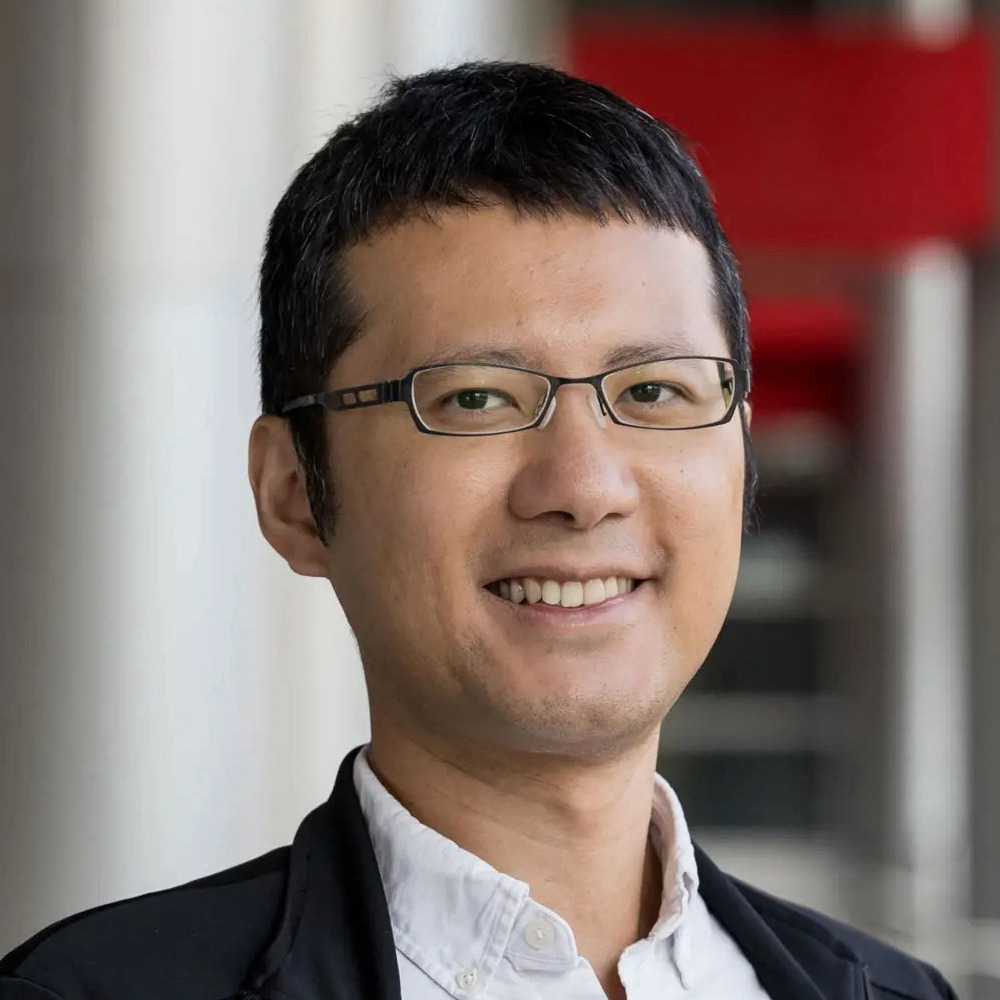
\includegraphics[width = 3cm]{twhuang_uwm.jpg}}; 
    \draw (0,0) circle (1.5cm);
    % if necessary the picture may be moved by changing the at (coordinates)
    % width defines the 'zoom' of the picture
\end{tikzpicture}
\hfill\vline\hfill
\end{minipage}
\begin{minipage}[c]{0.6\textwidth}
    \textbf{\Huge \scshape{ Tsung-Wei (TW) Huang}} \\ \vspace{2pt} 
    % \scshape sets small capital letters, remove if desired
    \small{} \\
    \href{mailto:tsung-wei.huang@wisc.edu}{\hspace{5pt} tsung-wei.huang@wisc.edu}\\
    % Be sure to use a professional *personal* email address
    % \href{https://www.linkedin.com/in/charles-rambo/}{\underline{linkedin.com/in/charles-rambo}} \\
    % you should adjust you linked in profile name to be professional and recognizable
    \href{https://tsung-wei-huang.github.io/}{\hspace{5pt} https://tsung-wei-huang.github.io/}
\end{minipage}

% Without picture
%\begin{center}
%    \textbf{\Huge \scshape Charles Rambo} \\ \vspace{1pt} %\scshape sets small capital letters, remove if desired
%    \small +1 123-456-7890 $|$ 
%    \href{mailto:you@provider.com}{\underline{you@provider.com}} $|$\\
%    % Be sure to use a professional *personal* email address
%    \href{https://linkedin.com/in/your-name-here}{\underline{linkedin.com/in/charles-rambo}} $|$
%    % you should adjust you linked in profile name to be professional and recognizable
%    \href{https://github.com/fizixmastr}{\underline{github.com/fizixmastr}}
%\end{center}



\begin{comment}
This CV was written for specifically for positions I was applying for in
academia, and then modified to be a template.

A standard CV is about two pages long where as a resume in the US is one page.
sections can be added and removed here with this in mind. In my experience, 
education, and applicable work experience and skills are the most import things
to include on a resume. For a CV the Europass CV suggests the categories: Work
Experience, Education and Training, Language Skills, Digital Skills,
Communication and Interpersonal Skills, Conferences and Seminars, Creative Works
Driver's License, Hobbies and Interests, Honors and Awards, Management and
Leadership Skills, Networks and Memberships, Organizational Skills, Projects,
Publications, Recommendations, Social and Political Activities, Volunteering.

Your goal is to convey a who, what , when, where, why for every item you share. 
The who is obviously you, but I believe the rest should be done in that order.
For example below. An employer cares most about the degree held and typically 
less about the institution or where it is located (This is still good 
information though). Whatever order you choose be consistent throughout.
\end{comment}

%-----POSITION----------------------------------------------------------------
\section{Appointment}
  \CVSubHeadingListStart
%    \CVSubheading % Example
%      {Degree Achieved}{Years of Study}
%      {Institution of Study}{Where it is located}
    \CVSubheading
      {{Associate Professor, Department of Electrical and Computer Engineering}}{2025 -- present}
      {University of Wisconsin at Madison, Madison, Wisconsin, USA}{}
    \CVSubheading
      {{Assistant Professor, Department of Electrical and Computer Engineering}}{2023 -- 2025}
      {University of Wisconsin at Madison, Madison, Wisconsin, USA}{}
    \CVSubheading
      {{Assistant Professor, Department of Electrical and Computer Engineering}}{2019 -- 2023}
      {University of Utah, Salt Lake City, Utah, USA}{}
    \CVSubheading
      {{Research Assistant Professor, Department of Electrical and Computer Engineering}}{2018 -- 2019}
      {University of Illinois at Urbana-Champaign, IL, USA}{}
    %     \CVItemListStart
    %     \CVItem{Major GPA 3.5/4 (CGPA 3.41)}
    %     \CVItem {Ranking 9/46 (top 20\%)}
    %   \CVItemListEnd
  \CVSubHeadingListEnd

%-----EDUCATION----------------------------------------------------------------
\section{Education}
  \CVSubHeadingListStart
%    \CVSubheading % Example
%      {Degree Achieved}{Years of Study}
%      {Institution of Study}{Where it is located}
    \CVSubheading
      {{PhD, Department of Electrical and Computer Engineering }}{2013 -- 2017}
      {University of Illinois at Urbana-Champaign, IL, USA}{}
    \CVSubheading
      {{MS, Department of Computer Science and Information Engineering}}{2010 -- 2011}
      {National Cheng Kung University, Tainan, Taiwan}{}
    \CVSubheading
      {{BS, Department of Computer Science and Information Engineering}}{2006 -- 2010}
      {National Cheng Kung University, Tainan, Taiwan}{}
    %     \CVItemListStart
    %     \CVItem{Major GPA 3.5/4 (CGPA 3.41)}
    %     \CVItem {Ranking 9/46 (top 20\%)}
    %   \CVItemListEnd
  \CVSubHeadingListEnd

%-----Research Interest--------------------------------------------
\section{Research Interest}
\textbf{Electronic Design Automation, High-performance Computing, Quantum Computing}{}
  

\section{Scientific Software Experience}
  {I create software systems to simplify the building of performance-critical applications. Many of them have been used by thousands of people from both industry and academia:}{}
  \CVSubHeadingListStart
    
    \CVSubheading
      {1. Taskflow: A General-purpose Parallel and Heterogeneous Programming System}{}
      {\url{https://taskflow.github.io/} (8--11K weekly downloads)}{}
      \CVItemListStart
        \CVItem{C++ Conference Best Poster Award, 2025 (voted by hundreds of C++ developers)}
        \CVItem{PPoPP FastCode Programming Challenge Winner (\nth{2} Place), 2025}
        \CVItem{MIT/Amazon/HPEC Graph Challenge Innovation Award (\nth{2} Place), 2023}
        \CVItem{MIT/Amazon/HPEC Graph Challenge Champion Award (\nth{1} Place), 2020}
        \CVItem{ACM Multimedia Best Open-source Software Award, 2019}
        \CVItem{C++ Conference Best Poster Award, 2018}
      \CVItemListEnd
    
    \CVSubheading
      {2. OpenTimer: A High-performance Timing Analysis Tool for VLSI Systems}{}
      {\url{https://github.com/OpenTimer/OpenTimer}}{}
      \CVItemListStart
        \CVItem{IEEE/ACM ICCAD 10-year Retrospective Most Influential Paper Award, 2024}
        \CVItem{ACM SIGDA Outstanding PhD Dissertation Award, 2019}
        \CVItem{Best EDA Software Tool, WOSET@ICCAD, 2018}
        \CVItem{Top-3 Winners of ACM TAU Contests, 2014--2016}
        \CVItem{Golden Timers of ACM TAU Contests, 2017--2021}
        \CVItem{Golden Timer of IEEE/ACM ICCAD CAD Contest, 2015}
      \CVItemListEnd
    
    \CVSubheading
      {3. DtCraft: A Data-parallel Distributed Streaming System}{}
      {https://github.com/twhuang-uiuc/DtCraft}{}
      \CVItemListStart
        \CVItem{ACM Multimedia Best Open-source Software Award, 2018}
      \CVItemListEnd
     
  \CVSubHeadingListEnd

% ------ Awards ------
\section{Selected Awards}
 \begin{itemize}
 \itemsep-3pt
    \item DAC Under-40 Innovator Award, 2025
    \item CoE Award for Excellence in Graduate Student Mentoring, UW-Madison, 2025
    \item ICCAD 10-year Retrospective Most Influential Paper Award, 2024
    \item \nth{2} Place, MIT/Amazon/HPEC Large Sparse Neural Network Challenge, 2023
    \item \nth{2} Place, MIT/Amazon/HPEC Streaming Graph Challenge, 2023
    \item ACM SIGDA Outstanding New Faculty Award, 2023
    \item ACM SIGDA Meritorious Service Award, 2022
    \item Humboldt Research Fellowship Award, Alexander von Humboldt Foundation, 2022
    \item Faculty Early Career Development Program (CAREER) Award, NSF, 2022
    \item \nth{1} Place, MIT/Amazon/HPEC Large Sparse Neural Network Challenge, 2020
    \item \nth{2} Place (Taskflow), Open-source Software Competition, ACM Multimedia Conference, 2019
    \item ACM SIGDA Outstanding PhD Dissertation Award (thesis title: ``Distributed Timing Analysis''), 2019
    \item Best Tool Award (OpenTimer), Workshop on Open-source EDA Technology, 2018
    \item Best Open-source Software Award (DtCraft), ACM Multimedia Conference, 2018
    \item Best Poster Award (Taskflow), CPP Conference, 2018
    \item \nth{2} and \nth{1} Place, ACM/SIGDA CADathlon International Programming Contest, 2014 and 2017
    \item \nth{1}, \nth{2}, and \nth{1} Place, ACM TAU Timing Analysis Contest, 2014--2016
    \item Yi-Min Wang and Pi-Yu Chung Endowed Research Award, ECE Dept. UIUC, 2016
    \item Rambus Computer Engineering Fellowship, ECE Dept. UIUC, 2015—2016
 \end{itemize}

% ------ PUBLICATION ------
\section{Selected Publication for My Scientific Software}
 \begin{enumerate}
 \itemsep-3pt
    
    \item \textbf{[ASPLOS'25]} Shui Jiang, Yi-Hua Chung, Chih-Chun Chang, Tsung-Yi Ho, and \underline{Tsung-Wei Huang}, ``BQSim: GPU-accelerated Batch Quantum Circuit Simulation using Decision Diagram,'' \textit{ACM International Conference on Architectural Support for Programming Languages and Operating Systems (ASPLOS)}, Rotterdam, Netherlands, 2025

    \item \textbf{[ICCAD'23]} Cheng-Hsiang Chiu, Dian-Lun Lin, and \underline{Tsung-Wei Huang}, ``Programming Dynamic Task Parallelism for Heterogeneous EDA Algorithms,'' \textit{IEEE/ACM International Conference on Computer-aided Design (ICCAD)}, San Diego, 2023
    
    \item \textbf{[IPDPS'23]} \underline{Tsung-Wei Huang}, ``qTask: Task-parallel Quantum Circuit Simulation with Incrementality,'' \textit{IEEE International Parallel and Distributed Processing Symposium (IPDPS)}, St. Petersburg, Florida, 2023 
  
  \item \textbf{[TPDS'22]} \underline{Tsung-Wei Huang}, Dian-Lun Lin, Chun-Xun Lin, and Yibo Lin, ``Taskflow: A Lightweight Parallel and Heterogeneous Task Graph Computing System,'' \textit{IEEE Transactions on Parallel and Distributed Systems (TPDS)}, vol. 33, no. 6, pp. 1303—1320, June 2022

    \item \textbf{[ICCAD'15]} \underline{Tsung-Wei Huang} and Martin D. F. Wong, ``OpenTimer: A High-performance Timing Analysis Tool,'' \textit{IEEE/ACM International Conference on Computer-aided Design (ICCAD)}, TX, 2015 (\textbf{2024 ICCAD 10-year Retrospective Most Influential Paper Award})

 \end{enumerate}

\section{Industrial Experience}
  \CVSubHeadingListStart
    \CVSubheading
      {{Software Engineer, High-performance Computing Group, Citadel, IL}}{May 2017 -- Aug 2017}
      {Developed machine learning benchmarks and optimization tips for financial workloads}{}
    \CVSubheading
      {{Software Engineer, Timing Analysis Group, IBM, NY}}{May 2015 -- Aug 2015}
      {Developed a distributed timing analysis prototype atop Einstimer}{}
    \CVSubheading
      {{Software Engineer, Timing Analysis Group, Mentor Graphics, CA}}{May 2014 -- Aug 2014}
      {Developed optimization algorithms for tag-based incremental timing analysis}{}
  \CVSubHeadingListEnd
    
\section{Miscellaneous}

\textbf{Citizenship:} Taiwan, US lawful permanent resident\\
\textbf{Hobby:} Piano playing, building better scientific software!
  
%-----Research Project--------------------------------------------
\begin{comment}
Again the title should have already been enough, but if it is necessary to add
descriptions maintain the consistency from prior sections
\end{comment}

%-----SE PROJECTS----------------------------------------------------
% \begin{comment}
% Ideally the title of the work should speak for what it is. However if you feel
% like you should explain more about why the project is applicable to this job,
% use item list as is shown in the work experience section.
% \end{comment}

% \section{Software Engineering Projects}
%   \CVSubHeadingListStart
% %    \CVSubheading
% %      {Title of Work}{When it was done}
% %      {Institution you worked with}{unused}
%     \CVSubheading
%       {{Iot Project on Smart Garden System built by ESP32} $|$ \emph{\small{C language}}}{Spring 2019}
%       {Xiamen University}{}
%     \CVSubheading
%       {{Big Data Analysis of Twitter} $|$ \emph{\small{Python}}}{Spring 2019}
%       {Xiamen University}{} 
%   \CVSubHeadingListEnd

%\section{Skills}
% \begin{enumerate}[leftmargin=0.5cm]
%    \small{\item{
%     \textbf{Languages}{: English (IELTS 6.5), Chinese (Native), Cantonese (Native)} \\
%     \textbf{Programming}{: Python (NumPy, SciPy, Matplotlib, Pandas), MATLAB, C \& C++, Java} \\
%     \textbf{Document Creation}{: Microsoft Office Suite, Latex, Markdown} \\
%    }}
% \end{enumerate}
    
%------------------------------------------------------------------------------
\end{document}
